\documentclass[fleqn,12pt]{article}
\addtolength{\hoffset}{-2cm} \addtolength{\textwidth}{4cm}
\addtolength{\voffset}{-2cm} \addtolength{\textheight}{4cm}
\usepackage{epsfig}
\usepackage[latin1]{inputenc}
\usepackage{float}
\usepackage{graphicx}
\usepackage{cancel}
\usepackage{mathrsfs}
\usepackage{amssymb}
\usepackage{amsfonts}
\usepackage{amsmath}
\usepackage{slashed}
\usepackage{indentfirst}

\usepackage{physics}

\usepackage{qcircuit}

% href
\usepackage{hyperref}


\newcommand{\eps}{\varepsilon}
\newcommand{\CC}{\mathbb{C}}
\newcommand{\RR}{\mathbb{R}}
\newcommand{\CZ}{\mathbf{CZ}}

\newcommand{\ts}{\tilde{*}}

\newtheorem{theorem}{Theorem}
\newtheorem{conjecture}{Conjecture}
\newtheorem{lemma}{Lemma}
\newtheorem{reduction}{Reduction}

\newenvironment*{proof}{\begin{trivlist}\item[]{\bf Proof.}}{\hfill$\square$\end{trivlist}}

% \usepackage{biblatex}

\pagestyle{empty}

\linespread{1.25}

\nocite{*}


\title{Translationally Invariant Random Quantum Circuits}
% \subtitle{8.371 Spring 2023 Final Paper}
\author{Rowechen Zhong}

\begin{document}
\maketitle
\section{Abstract}
Random quantum circuits have a wide range of applications,
spanning from quantum computing and quantum many-body systems
to the study of black holes in physics. In quantum information science,
their usages abound \cite{Hayden_2004};
they are ubiquitous in protocols for transferring information through quantum channels,
quantum data-hiding, encryption, and information locking.

The gold standard for the generation of pseudorandom unitaries is the Haar
measure, which is the natural ``uniform" distribution over unitary matrices.
The natural way to quantify how close a given distribution is to the Haar measure,
is through the notion of ``approximate $k$-designs;'' a distribution is a $k$-design if
it has $k$-th moments equal to those of the Haar distribution.

Significant progress has been made on this front in the past few years.
In 2005, Emerson et al. \cite{Emerson_2005} showed that random quantum circuits
in fact converge to the Haar measure.
In 2009, Harrow and Low \cite{Harrow_2009} showed that random circuits of
polynomial length are approximate $2$-designs. In 2019, Brand{\~{a}}o et al. \cite{Brand_o_2016}
showed that in fact, \emph{nearest-neighbor} two-qubit gates are sufficient
to form approximate unitary $t$-designs. Specifically, they studied the circuit formed by
interleaving $2$-qubit unitaries in a ``brickwork architecture.''
Their work represented a significant amalgamation
of mathematical theory, incorporating quantum many-body theory, representation theory, and
the theory of stochastic processes. Finally, in August 2022, Haferkamp \cite{Haferkamp_2022}
reduced the constant factors required by their construction significantly.

When Brand{\~{a}}o et al. specialized to the brickwork architecture, they introduced a
degree of \emph{locality} into the problem. In particular, the local entanglement caused by
geometrically adjacent two-qubit gates was shown to be sufficient to form global entanglement
across the entire system. This specialization was physically and practically motivated.
Quantum hardware is typically designed to allow robust operations between neighboring qubits.
Studying such random circuits may also yield interesting insights into the nature of physical
systems, as modeled using local interactions on a lattice.

In this paper, we will study variations of this question, which are also physically motivated.
One direction is to consider the limiting distribution of a series of \emph{symmetric}
entangling operators on a circle of $N = 2n$ qubits. We will perform the
\emph{same} Haar-random unitary on pairs of adjacent qubits, in a brickwork architecture.
% on each qubit, followed by
% a standardized entangling operation, Controlled-Z, on each edge of the graph.
% Depending on the feasibility of the problem, we may consider either a fully-connected graph,
% or a cycle.
It is a well-known paradigm that symmetries in a system yield conservation laws;
in this case, one would expect that the symmetries yield nontrivial subspaces preserved by
all operations; then the distribution is expected to converge to some (presumably Haar-random)
distribution across each subspace.

% An alternative direction is to analyze the limiting distribution of this series of entangling
% operators, with arbitrary randomly selected unitary operations, over an arbitrary graph.
% This direction may be pursued if the former is too difficult.
% In all cases, we may restrict attention
% to \emph{infinitesimal} operations, where the unitaries are randomly chosen from some suitable
% small $\epsilon$-neighborhood of the identity, and $\epsilon$ is taken to $0$.

We will refer to Fulton's textbook \cite{fulton_harris_2004} and \cite{Etingof2009} as a
reference for representation theory.

\section{Background}

Consider the unitary group $U(D)$ over a dimension-$D$ Hilbert space.
Suppose you wanted to design a uniform measure $\mu$ for the
Borel algebra $\mathcal{B}(U(D))$. Such a measure ought to be invariant under
actions by elements of $U(D)$;
\[
    \mu(gS) = \mu(S),\qquad \forall g \in U(D), S \in \mathcal{B}(U(D))
\]

It turns out that such a distribution is essentially \emph{unique}, after imposing
some sanity conditions: inner and outer regularity and finiteness on compact sets.
The resulting measure is called the \emph{Haar measure} on $U(D)$.
% $U(D)$, being a locally compact Hausdorff topological group, has a unique

The subject of this paper is the following random circuit:

% \begin{align}
\begin{figure}[H]
    \centerline{
    \Qcircuit @C=0.75em @R=2em {
    \lstick{\vdots }       &     &                    & \multigate{1}{W_1} &                    & \multigate{1}{W_2} & \cdots \\
    \lstick{\ket{x_2}}     & \qw & \multigate{1}{U_1} & \ghost{W_1}        & \multigate{1}{U_2} & \ghost{W_2}        & \cdots \\
    \lstick{\ket{x_1}}     & \qw & \ghost{U_1}        & \multigate{1}{W_1} & \ghost{U_2}        & \multigate{1}{W_2} & \cdots \\
    \lstick{\ket{x_0}}     & \qw & \multigate{1}{U_1} & \ghost{W_1}        & \multigate{1}{U_2} & \ghost{W_2}        & \cdots \\
    \lstick{\ket{x_{N-1}}} & \qw & \ghost{U_1}        & \multigate{1}{W_1} & \ghost{U_2}        & \multigate{1}{W_2} & \cdots \\
    \lstick{\ket{x_{N-2}}} & \qw & \multigate{1}{U_1} & \ghost{W_1}        & \multigate{1}{U_2} & \ghost{W_2}        & \cdots \\
    \lstick{\vdots }       &     & \ghost{U_1}        &                    & \ghost{U_2}        &                    & \cdots
    }
    }
    \caption{Translation-Invariant Brickwork Architecture}
\end{figure}
% \end{align}

We conceptualize there being $N = 2n$ qubits total, with qubits enumerated modulo $N$,
such that the network is entirely symmetric under rotation by $2$ qubits.
On layer $k$, two random
two-qubit unitaries $U_k, W_k \in U(4)$ are sampled from the Haar measure.
For notation, for any two-qubit unitary $U$,
let $U(a, b)\in U(2^N)$ denote the action of $U$ on qubits $a$ and $b$.
We then apply $U(2m, 2m+1)$ for all $m$, followed by $W(2m+1, 2m+2)$ for all $m$.
Let $M_k \in U(2^N)$ denote the entire unitary enacted by layer $k$, and
let $T_k\in U(2^N)$ denote the entire unitary consisting of the product of all operators up to layer $k$.

Each $U_k, W_k$ is a random variable, and thus so is $T_k$.
The goal of this paper is to analyze the
limiting distribution of $T_k$ as $k \to \infty$.


We define the \emph{rotation operator} $\mathcal{R}$ by its action on
pure tensors;
\[
    \mathcal{R} \ket{a_1 a_2 \cdots a_N} = \ket{a_3 a_4\cdots a_N a_1 a_2}
\]
and extend by linearity. Define the \emph{rotation superoperator} $\mathfrak{R}$ as
\[
    \mathfrak{R}(U) = \prod_{i = 1}^n \mathcal{R}^i U \mathcal{R}^{-i}
\]
Thus,
\[
    M_k = \mathfrak{R}(U_k(0,1)) \mathfrak{R}(W_k(1,2))
\]

The motivation behind our main theorem is the following series of observations:
\begin{lemma}
    $\mathcal{R}$ commutes with $\mathfrak{R}(U)$ for all $U\in U(2^N)$.
\end{lemma}
\begin{proof}
    \[
        \mathcal{R} \mathfrak{R}(U) = \mathcal{R} \prod_{i = 1}^n \mathcal{R}^i U \mathcal{R}^{-i}
        = \prod_{i = 1}^n \mathcal{R}^{i+1} U \mathcal{R}^{-i} = \mathfrak{R}(U)\mathcal{R}
    \]
\end{proof}
We will forever let $\omega_n = e^{2\pi i / n}$.

$\mathcal{R}^n = 1$, thus $\mathcal{R}$ has eigenvalues $\omega_n^k$ for
$k = 0, 1, \ldots, n-1$.
Let $V_k \subset \CC^{2^N}$ be the $\omega_n^k$-eigenspace of $\mathcal{R}$,
for $k = 0, 1, \ldots, n-1$.
Then, by the previous lemma, each eigenspace is left
invariant by all $\mathfrak{R}(U)$; in particular,
each eigenspace is left invariant by $T_k$ for all $k$.
Thus, the limiting distribution consists of unitary matrices
that are \emph{block-diagonal} in any basis respecting $V_k$.

\begin{lemma}
    We can write down a complete set of orthonormal projectors
    onto each $V_k$;
    \[
        P_k = \frac{1}{n}\sum_{i = 0}^{n-1} \omega^{-ik} \mathcal{R}^i
    \]
\end{lemma}
\begin{proof}
    This is essentially clear;
    \begin{align*}
        P_k P_\ell & = \frac1{n^2} \sum_{0\leq i,j < n} \omega^{-ik} \omega^{-j\ell} \mathcal{R}^{i+j}
        = \frac1{n^2} \sum_{0\leq i,j < n} \omega^{-i(k - \ell)} \omega^{-(i + j)\ell} \mathcal{R}^{i + j}                           \\
                   & = \frac1{n^2} \sum_{0\leq i,j < n} \omega^{-i(k - \ell)} \omega^{-j\ell} \mathcal{R}^j  = \delta_{k\ell} P_\ell
    \end{align*}
    and
    \[
        \sum_{k = 0}^{n-1} P_k = \frac1n \sum_{k = 0}^{n-1} \sum_{i = 0}^{n-1} \omega^{-ik} \mathcal{R}^i
        = \mathcal{R}^0 = I
    \]
    $P_k$ leaves $\omega$-eigenspace $V_k$ invariant, since for any $v\in V_k$,
    \[
        P_k v = \frac{1}{n} \sum_{i = 0}^{n-1} \omega^{-ik} \mathcal{R}^i v
        = \frac{1}{n} \sum_{i = 0}^{n-1} \omega^{-ik} \omega^{ik} v = v
    \]
    (similarly they kill $V_\ell$ for $\ell \neq k$). They are clearly Hermitian.
\end{proof}
Clearly, $P_k$ commutes with all $\mathfrak{R}(U)$; they
can be pulled to the front of all expressions.
All we're trying to do is single out an eigenspace.

Let $\mathcal{M}^{(k)}$ be all elements of the form $M P^k$,
where $M = \mathfrak{R}(U(0,1)) \mathfrak{R}(W(1,2))$
as usual.

By abuse of notation, we will sometimes consider $P_k$ as a map $V\to V_k$
by inclusion; the risk of confusion is minimal.

Thus, we have our blocks: for each $0\leq k < n$, let
$M_t^{(k)} = M_t P^k$ and
$T_t^{(k)} = T_t P^k$ be operators over $U(V_k)$ (unitary operators
which are nonzero only in the $V_k$ block).
By block-diagonality, it is clear that
\[
    T_t = T_t^{(0)} \oplus \cdots \oplus T_t^{(n-1)},\qquad T_t^{(k)} = M_1^{(k)} M_2^{(k)} \cdots M_t^{(k)}
\]

This motivates:
\begin{theorem}
    [Main Theorem]
    For each $0\leq k < n$, as $t\to \infty$, $T_t^{(k)}$
    converges uniformly to
    the Haar distribution over $U(V_k)$.
\end{theorem}

While we do not prove this theorem, it will be reduced to a combinatorial problem,
which is amenable to algorithmic simulation.

\section{Measure Theory}

Let $\mathcal{F}$ denote the set of probability measures over $U(V_k)$.
$M^{(k)}_t$ is drawn at random from some complicated
measure which we will call $f\in \mathcal{F}$.

Then, the distribution of $T^{(k)}_t$ is naturally described via convolution;
\[
    P(T^{(k)}_t = g) = \underbrace{f * f * \cdots f}_{k\text{ times}}
    = \int d \mu(h_{t-1})\cdots d \mu(h_1) f(gh_{t-1}^{-1})\cdots f(h_2 h_1^{-1}) f(h_1)
\]
where $d \mu(g)$ is the Haar measure over $U(D)$.


The following intuitive theorem is due to
Emerson et al.\cite{Emerson_2005}, and saves us from tangling
too much with measure theory.
\begin{theorem}
    [Generation implies convergence]
    Suppose $f$ is a probability measure over the compact Lie group $U(D)$.
    If $f$ has support on a subset of $U(D)$ that generates $U(D)$,
    then $f^{*m}$ converges uniformly to the Haar measure on $U(D)$.
\end{theorem}

The theorem is natural, because if $f^{*m}$ converges, then it clearly
must converge to the Haar measure; the trick
is to show that it converges at all.

In any case, we have our first reduction:
\begin{reduction}
    [Generation]
    The main theorem follows if $f$ has support on a subset of $U(V_k)$
    that generates $U(V_k)$.

    In particular, call the subgroup generated by $\mathcal{M}^{(k)}$
    $\mathcal{S}\subset U(V_k)$; the claim is that $\mathcal{S} = U(V_k)$.

    % In other words, the theorem follows if, for any element $U(V_k)$, there exists $t$ and 
    % a sequence $U_1,\cdots U_t$ and $V_1\cdots V_t$ such that
    % \[
    %     P_k \mathfrak{R}(U_1(0,1) NP_0 W_1(1,2) NP_0 \cdots NP_0 U_k(0,1) NP_0 W_k(1,2))
    % \]
\end{reduction}

\section{Lie Algebra}

The space of unitary matrices is pretty complicated. The associated \emph{Lie algebra},
which consists of \emph{infinitesimal} unitaries, is much easier to handle.

$U(D)$ is a compact and simply connected Lie group; as such, there is a well-known correspondence
via the exponential map $\exp : \mathfrak{u}(D) \to U(D)$ is $U(D)$
that maps $\mathfrak{u}(D)$ surjectively over $U(D)$. Keep in mind that all lie algebras
described are \emph{real}. Thus, it would suffice to show that infinitesimal elements
of $\mathcal{M}^{(k)}$ generate the
lie algebra of $U(V_k)$.


We will now be making extensive use of the (generalized) Pauli matrices:
\[
    I = \begin{pmatrix}
        1 & 0 \\ 0 & 1
    \end{pmatrix},\qquad
    X = \begin{pmatrix}
        0 & 1 \\ 1 & 0
    \end{pmatrix},\qquad
    Y = \begin{pmatrix}
        0 & -i \\ i & 0
    \end{pmatrix},\qquad
    Z = \begin{pmatrix}
        1 & 0 \\ 0 & -1
    \end{pmatrix}
\]
which are also called $\sigma^0, \sigma^1, \sigma^2, \sigma^3$ respectively;
and $\sigma^s = \sigma^{s_0}\cdots \sigma^{s_{n-1}}$ for $s\in \{0,1,2,3\}^n$.


Well, we can easily write down the infinitesimal generators
of $\mathcal{M}^{(k)}$, which we identity with the lie algebra
$\mathfrak{M}^{(k)}$:
when $U = I + iA$, $T = I + iB$ with $A,B$ infinitesimal
hermitian $2\times 2$ matrices,
\begin{align*}
    M & = \prod_{i = 1}^n \mathcal{R}^i U(0,1) \mathcal{R}^{-i} \prod_{j = 1}^n \mathcal{R}^j T(1,2) \mathcal{R}^{-j} P_k \\
      & = P_k + P^\dagger_k\sum_{i = 1}^n \mathcal{R}^i\left(iA(0,1) + iB(1,2)\right) \mathcal{R}^{-i} P_k                \\
      & = P_k + P^\dagger_k\left(iA(0,1) + iB(1,2)\right) P_k \tag{$\star$}
\end{align*}
Clearly, $A,B$ can be taken to be $2$-qubit Pauli strings.

More infinitesimal elements of $M$ can be generated through
linear operations and the lie bracket (the commutator).
Let $\mathcal{H}(D)$ denote the $D\times D$ hermitian matrices.
Observe that for any $A,B\in \mathcal{H}(2^N)$,
\[
    [P^\dagger_k iA P_k, P^\dagger_k iB P_k]
    = P^\dagger_k 2i\underbrace{\frac{1}{2i}\left(\sum_j A \mathcal{R}^j B \mathcal{R}^{-j}
        - \mathcal{R}^j B\mathcal{R}^{-j}  A\right)}_{A \ts B} P_k
\]
This motivates the definition of the \emph{convolution commutator}:
\[
    A \ts B = \frac{1}{2i}\left(\sum_j A \mathcal{R}^j B \mathcal{R}^{-j}
    - \mathcal{R}^j B\mathcal{R}^{-j}  A\right)
\]
It will soon be clear why this is an appropriate name.

$\mathfrak{u}(2^N)$ consists of the $2^N\times 2^N$ antihermitian matrices,
which can be identified with linear combinations of
Pauli strings of length $N$. To distinguish the basis elements
(individual Pauli strings)
from linear combinations of Pauli strings, I will use the adjective ``pure.''
An arbitrary example is
\[
    iX\otimes Y\otimes Z \in \mathfrak{u}(2^3)
\]

Thus, the infinitesimal elements of $U(V_k)$ are simply
\[
    i P_k \sigma^s P_k
\]

All we need to do is show that we can create all elements of the above form using
linear combinations and commutators of $\star$.
Dropping the wrapping $P_k$'s and the $i$ prefactor,
we produce our next reduction.
\begin{reduction}
    [Lie Generation]
    \label{reduction:lie-generation}
    The following implies the main theorem.

    Suppose there exists a (real) linear subspace $S\subset \mathcal{H}(2^N)$ such that:
    \begin{enumerate}
        \item For any hermitian $A\in U(4)$, $A(0,1), A(1,2) \in S$.
        \item For any $X, Y \in S$, $X \ts Y \in S$.
        \item For any $X \in S$, $\mathcal{R} X \mathcal{R}^{-1} \in S$.
    \end{enumerate}
    Then, $S = \mathcal{H}(2^N)$.
\end{reduction}

\section{Combinatorics}

Item (3) of the previous reduction means we only care about
the generated operators up to equivalence classes under rotation. Thus, we present
the following notation, which is best explained with examples in the $n = 3$
case:
\begin{align*}
    Xx     & \equiv \{ XXIIII, IIXXIIX, IIIIXX \} \\
    Xy     & \equiv \{ XYIIII, IIXYII, IIIXYI \}  \\
    xX     & \equiv \{ IXXIII, IIIXXI, XIIIIX \}  \\
    XiZ    & \equiv \{ XIZIII, IIXIZI, ZIIIXI \}  \\
    XiXiXi & \equiv \{ XIXIXI\}
\end{align*}

Explicitly: we only care about elements up to rotation by $2$ qubits;
capital letters denote even indices and lowercase letters denote odd indices;
leading and trailing $I$'s are omitted.

Here is what a generic convolution commutator looks like:
\[
    Xx \ts yZ = \frac{1}{2i}[XXIIII, IYZIII + IIIYZI + ZIIIIY] = XZZIII + 0 - YXIIIY = XzZ - yYx
\]
It is now apparent that the $\frac1{2i}$ factor was chosen to kill the
irrelevant global phase factors that will always occur in such a commutation.

For hand-calculation of these convolution commutators, several things quickly
become apparent:
\begin{itemize}
    \item The background $I$'s commute with everything;
          thus they can safely be ignored.
    \item In order for two Pauli strings to \emph{fail} to commute,
          they must differ in an odd number of entries.
    \item Global phase factors of $\pm 1$ can be dropped, but one must
          remain vigilant for local phase flips.
\end{itemize}
And the following lemma:
\begin{lemma}
    [Symmetric Constructions]
    $X, Y, Z$ are essentially symmetric. In addition, there is
    symmetry about reversing all strings, and translating by $1$ unit.
    Thus, after finding $XxY\in S$, we immediately know
    $YyX, YyZ, xZz, \cdots \in S$.
\end{lemma}

In order to prove a statement like \ref{reduction:lie-generation},
one would have to design an algorithm that, given a Pauli string, generates a sequence of convolution
commutations evaluating to the Pauli string.

While I was unable to design such an algorithm, we offer
some constructions that may eventually
lead to such an algorithm.

One insight is that there are two possible ways this algorithm could conceivably
work: a \emph{local} method, and a \emph{global} method. A local method only
ever requires strings that are of bounded length in order to create a pauli string of fixed length;
in other words, to create the string $XyZ$ when $N = 10^{10}$, one would not
have to create strings of length $O(N)$
as intermediate steps. In contrast, a global method is significantly more complex,
making use of the finiteness of $N$, such that convolutions must wrap around the
circle of qubits to construct desired Pauli strings.

\begin{figure}[h]
    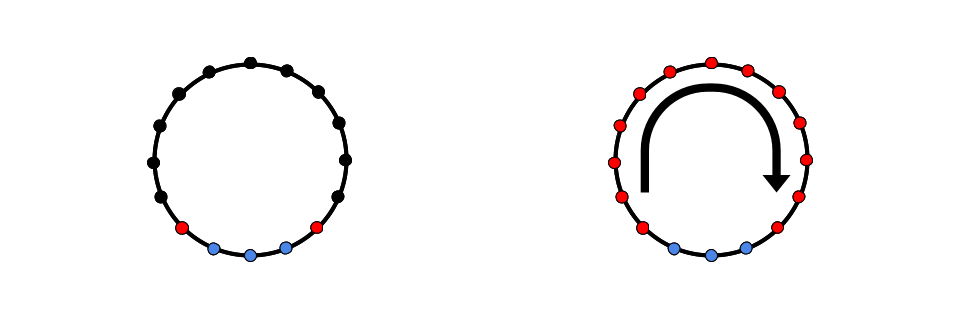
\includegraphics[width = \textwidth]{Untitled drawing.png}
    \caption{A ``local'' method (left) would only interact with a bounded number of qubits
        (red) in order to construct a desired Pauli string (blue). A ``global'' method (right)
        would have to wrap around the circle of qubits to construct a desired Pauli string.}
\end{figure}


Unfortunately, through numerical simulations as described later, I have been unable
to construct the simple string $XyZ$ locally. Thus, we present a global construction
that may facilitate the construction of a global algorithm.

\begin{theorem}
    [Chains]
    It is possible to form arbitrarily long chains of the form $XzZ\cdots ZzX$
    and $XzZ\cdots zZy$ (whose length is bounded by $N$).
    In particular, one can create a chain $Zz\cdots Z$ of length $N - 1$.
\end{theorem}
\begin{proof}
    Begin with $Xx \ts yX = XzX$. Then, $XzX \ts Yy = XzZy$.
    Continuing, $XzZy \ts yY = yZzZy$; this is symmetric to $XzZzX$.
    Apply $Yy$ again, ad nauseam, to yield strings $XzZ\cdots ZzX$
    and $XzZ\cdots zZy$.

    We eventually reach $XzZ\cdots ZzX$ of length $N - 1$:
    \begin{align*}
        \cdots ZzZz\underbrace{XiXz}ZzZ\cdots
    \end{align*}
    Applying $Yy$ as usual, we find
    \[
        \cdots ZzZz\underbrace{ZyXz}ZzZ\cdots
    \]
    Applying $yY$ one last time, we achieve
    \[
        \cdots ZzZz\underbrace{ZiZz}ZzZ\cdots
    \]
    as desired.
\end{proof}

Previously, all strings were padded by $I$'s on both sides;
this construction shows that we can change the ``background''
we choose to work in to be $Z$'s instead of $I$'s.

This substrate is significantly more reactive than $I$'s;
attempting to use this construction combined with local constructions
tends to cause large amounts of anticommutations to occur at once,
rendering hand calculations difficult.

\section{Computer Analysis}

\subsection{Methods}

For any finite $n$, the approach is straightforward; there are a finite
number of pauli strings to generate, so we just enumerate all pauli
strings through brute force. Specifically, the dimension of our space is
simply $4^N$, and pauli strings can be naively encoded as vectors in $\RR^{4^N}$.
I call this method of encoding the algebra
the \emph{vector method}.

Of course, this takes exponential time. Thus I implemented the following optimizations:
\begin{itemize}
    \item Only consider equivalence classes of pauli strings under shifts by $2$ qubits.
          Automatically include the symmetric constructions under the lemma.
    \item While general elements of our algebra are linear combinations of pauli
          strings, significant progress can be made by restricting ourselves to pure
          pauli strings. This is done for as long as possible;
          then operations like checking for linear independence become trivial
          (using a hash table). I call this method of encoding the algebra
          as the \emph{dictionary method}.
    \item Originally, I attempted to check linear independence through singular-value
          decomposition. This proved to be too slow, so I switched to using the QR decomposition.
\end{itemize}

In addition, while attempting to discover a local algorithm, I worked
in the context of ``unbounded'' pauli strings; we imagine $N\to \infty$
such that we never have to consider convolutions that wrap around.

\subsection{Results}

If we count by groups of two qubits, there are three possible types
of $6$-qubit pauli strings:
\begin{itemize}
    \item $AAA$, of which there are $16$.
    \item $AAB$, of which there are $16 \cdot 15 = 240$.
    \item $ABC$, of which there are $16 \cdot 15 \cdot 14 / 3 = 1120$.
\end{itemize}
In total, there are $1376$ distinct pauli
strings up to cyclic rotations.

Unfortunately, both the vector and dictionary methods were unable
to enumerate all $1376$ distinct pauli strings in $6$-qubit case; only $1374$
were found. The $8$-qubit case appears to be too large to
feasibly simulate on computational resources I have access to,
even with all the accelerations above.

All code can be found on github at
\href{https://github.com/rowechenzhong/QIS-Project}{github.com/rowechenzhong/QIS-Project}.

In addition, in the unbounded case was able to produce
a large list of pauli strings, which can be used for any $N$ due
to their local nature. Some small examples of pure states we can generate include:
\begin{align*}
    XxX, XyX, XyZz, XxYy, XyYz,XyZx, XxYxX,\cdots
\end{align*}

Note that we are missing local constructions for two simple $3$-qubit
interactions, $XyZ$ and $XxY$. Indeed, although we can
form many linear combinations of $3$-qubit interactions
such as $XyY -zZx  = zY  \ts  Xx$, these do not span
the space of $3$-qubit interactions.
In retrospect, this is expected.

\section{Conclusion}

The most immediate extension of this work would be to
discover a general construction for all pauli strings.
After this, one could begin work on the convergence
properties of our quantum circuit; in particular, we might
ask whether it converges to an $t$-design at the same rate
as previous work \cite{Brand_o_2016}\cite{Haferkamp_2022}.

In addition, by restricting ourselves to work in
subspaces of the full space of operators, we ignored possible
correlations that would occur \emph{between} the subspaces --
it is clearly not true in general that a joint distribution
is completely determined by its marginals. Thus, while I do not
expect there to be a ``clean'' answer in this case, additional
studies on the mixing between the $V_k$ subspaces would be interesting.

Finally, observe that the graph structure of our qubits is a \emph{directed}
$2n$-cycle, with symmetry group $C_n$. At the beginning of this project,
I worked extensively on the
case of the \emph{undirected} $n$-cycle, which may naively seem easier.

%\begin{align}
%\end{align}

Here, the vertical lines are controlled-$Z$ gates, our sole (symmetric)
entangling operation. Unfortunately, I soon came to realize that the
symmetry group of this circuit is not $C_n$, but rather the dihedral group
$D_n$; the circuit is invariant under $x_{i}\to x_{n+1-i}$. Importantly,
$D_n$ is \emph{not} abelian. This seemingly innocuous detail destroys
our theorem. Our existing $V_k$ subspaces are still
invariant (where $V_k$ are eigenspaces under rotation by $1$ qubit).
However, one can define two additional subspaces $W_+$ and $W_-$, which
are the eigenspaces under \emph{reflection} about the axis
passing through qubit $\ket{x_0}$. These subspaces do not intersect
nicely with the $V_k$ subspaces; it is a general fact of linear algebra
that in a dimension $N$ vector space, two subspaces of size $a,b$ need
not intersect at all if $a + b \leq N$.


\begin{figure}[H]
    \centerline{
    \Qcircuit @C=0.75em @R=2em {
    \lstick{\vdots }       &     &           &           &               &           &           &     & \\
    \lstick{\ket{x_1}} & \qw & \ctrl{1}  & \gate{U_1}& \ctrl{1}      & \gate{U_2}& \ctrl{1}  & \qw & \\
    \lstick{\ket{x_0}}     & \qw & \ctrl{-1} & \gate{U_1}& \ctrl{-1}     & \gate{U_2}& \ctrl{-1} & \qw & \\
    \lstick{\ket{x_{-1}}} & \qw & \ctrl{-1} & \gate{U_1}& \ctrl{-1}     & \gate{U_2}& \ctrl{-1} & \qw & \\
    \lstick{\ket{x_{-2}}} & \qw & \ctrl{-1} & \gate{U_1}& \ctrl{-1}     & \gate{U_2}& \ctrl{-1} & \qw & \\
    \lstick{\vdots }       &     &           &           &               &           &           &     &
    }
    }
    \caption{Cyclically Symmetric Circuit}
\end{figure}


Thus, the $D_n$ case is significantly more complicated than the $C_n$ case.
The analogous statement of our main theorem is \emph{wrong} for $n = 3$
where $D_6 = S_3$ is nonabelian.
In the language of graph theory, the \emph{automorphism group} of the
undirected $n$-cycle is nonabelian.

However, this yields a natural question: does our above analysis extend
to arbitrary graphs with abelian automorphism groups? There are
many such graphs of interest.

\begin{figure}[H]
    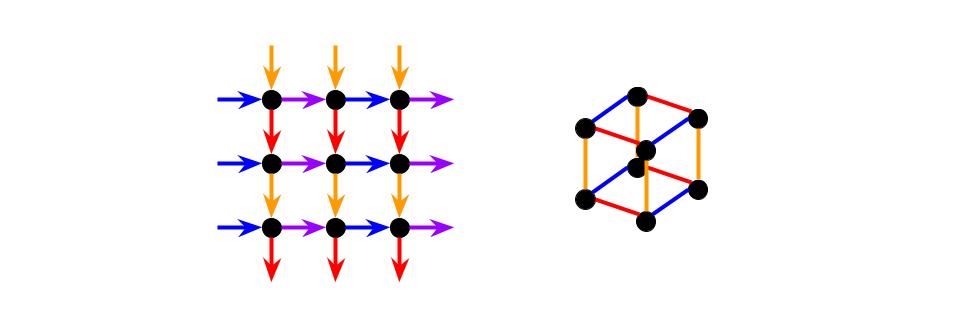
\includegraphics[width = \textwidth]{Automorphism.png}
    \caption{The graph on the left is a section of a colored, directed graph.
    The graph is understood to eventually wrap around on the left and right, as
    well as top and bottom, such that it forms a torus. If there are $2m\times 2n$
    qubits (vertices) in the graph, then the automorphism group is $C_m\oplus C_n$,
    an abelian group. The undirected graph on the right is a hypercube of dimension $D = 3$.
    The automorphism group is $C_2^{\oplus D}$, also an abelian group.}
\end{figure}


\begin{conjecture}
    [Informal]
    Given some (possibly directed, or colored) graph $G$ with
    abelian automorphism group,
    one can construct a quantum circuit whose qubits are identified
    with the vertices and whose gates are identified with the edges.

    The gates are arranged into layers. On each layer, to each color
    of edge, we apply the \emph{same} randomly chosen unitary operation.
    This is possible to do simultaneously so long as no two edges
    of the same color share a vertex.

    As this procedure is taken to the limit, the entire unitary enacted
    on this circuit approaches some limiting distribution.

    It is easy to see that such a limiting distribution must block-diagonalize
    into the subrepresentations of the automorphism
    group. Does it converge to a Haar distribution on each block?
\end{conjecture}

The well-known \emph{structure theorem for finite abelian groups} states
that any finite abelian group $G$ is isomorphic to a direct product of
cyclic groups, which was precisely the case studied in this paper.
Perhaps future work may reveal the relationship between these two cases.

\section{Acknowledgements}

I would like to thank Professor Soonwon Choi for his phenomenal Quantum
Information Science course, and for suggesting this topic to me.
I learned lots of quantum computing from Michael
Nielson and Isaac Chuang's \emph{Quantum Computation and Quantum
    Information} textbook, which is a good resource.


% \section{Day 1 Progress}

% Today, I investigated the $n = 2$ qubit case; $N = 2^n = 4$.

% Explicitly: begin with the $M_0 = I_N$ identity matrix on $\CC^N$.
% On step $i$, pick a random $T\in U(2)$ over the Haar measure.
% Then, let $M_{i+1} = \CZ T^{\otimes 2} M_i$, where
% $\CZ$ is the controlled-Z gate.
% \[
%     \CZ = \begin{pmatrix}
%         1 & 0 & 0 & 0  \\
%         0 & 1 & 0 & 0  \\
%         0 & 0 & 1 & 0  \\
%         0 & 0 & 0 & -1
%     \end{pmatrix}
% \]

% It is immediately clear that there are two disjoint subspaces
% left invariant under this action: the \emph{symmetric subspace}
% spanned by $\ket{00}, \ket{11}, \frac{1}{\sqrt2} (\ket{01} + \ket{10})$,
% and the \emph{antisymmetric subspace} spanned by
% $\frac{1}{\sqrt2} (\ket{01} - \ket{10})$.

% We explicitly calculate the evolution $\CZ T^{\otimes 2}$ for
% \[
%     T = \begin{pmatrix}
%         a & b \\
%         c & d
%     \end{pmatrix},\qquad \abs{a}^2 + \abs{b}^2 = \abs{c}^2 + \abs{d}^2 = 1,\qquad ac^* + bd^* = 0.
% \]
% in the basis $\{\ket{00}, \ket{11}, \frac{1}{\sqrt2} (\ket{01} + \ket{10}), \frac{1}{\sqrt2} (\ket{01} - \ket{10})\}$.
% \[
%     C_Z T^{\otimes 2} = \begin{pmatrix}
%         a^2        & ab\sqrt{2}  & b^2        & 0     \\
%         ac\sqrt{2} & ad + bc     & bd\sqrt{2} & 0     \\
%         -c^2       & -cd\sqrt{2} & -d^2       & 0     \\
%         0          & 0           & 0          & ad-bc
%     \end{pmatrix}
% \]

% It has the block-diagonal structure as claimed. In particular, the antisymmetric subspace
% clearly experiences random elements of $U(1)$; the determinant of a random selected element of $U(2)$
% over the Haar measure will be Haar on $U(1)$ (which be easily proven
% using methods from \cite{Collins_2006}).

% We now consider the limiting distribution of the projection of $M_{i+1}$ onto the symmetric subspace.
% We claim that it converges to the Haar distribution. To this end, we use the following
% completely natural result:
% \begin{theorem}
%     [Generation implies convergence]
%     \cite{Emerson_2005}
%     Suppose $f$ is a probability measure over the compact Lie group $U(D)$.
%     If $f$ has support on a subset of $U(D)$ that generates $U(D)$,
%     then $f^{*m}$ converges uniformly to the Haar measure on $U(D)$.
% \end{theorem}

% This simply states that, being the natural uniform distribution, as long as
% we can generate all elements of $U$, the limiting beaviour of compositions
% will be Haar.

% It suffices to generate the infinitesimal elements of $U(3)$ using blocks of the following form:
% \[
%     \begin{pmatrix}
%         a^2        & ab\sqrt{2}  & b^2        \\
%         ac\sqrt{2} & ad + bc     & bd\sqrt{2} \\
%         -c^2       & -cd\sqrt{2} & -d^2
%     \end{pmatrix}
% \]
% Well, allow $a = d = 1$ and $\abs{b}, \abs{c} < \eps  \ll 1$; the unitarity condition is $b = -c^*$.
% Absorbing the factor of $1/\sqrt2$ into $b$, we have
% To first order, we have
% \[
%     \begin{pmatrix}
%         1 & b  & 0  \\
%         c & 1  & b  \\
%         0 & -c & -1
%     \end{pmatrix} + O(\eps^2)
% \]
% Multiplying by an analogous matrix,
% \[
%     \begin{pmatrix}
%         1 & b  & 0  \\
%         c & 1  & b  \\
%         0 & -c & -1
%     \end{pmatrix}
%     \begin{pmatrix}
%         1 & x  & 0  \\
%         y & 1  & x  \\
%         0 & -y & -1
%     \end{pmatrix}
%     = \begin{pmatrix}
%         1     & b + x & 0   \\
%         c + y & 1     & x-b \\
%         0     & y-c   & 1
%     \end{pmatrix} + O(\eps^2)
% \]
% Thus we can generate any infinitesimal unitary among the first two qubits and
% among the second two qubits. This suffices to generate all unitaries in $U(3)$.

% Notes on how I expect to analyze the general case.
% \begin{itemize}
%     \item This is correctly formulated as a question about some sort of representation;
%           $U(2)$ in $\CC^{N}$ via
%           \[
%               T\to T^{\otimes n}
%           \]
%     \item Then, in some sense, I need to determine the ``invariant subspaces'' of this
%           representation that are ``simulatanously invariant'' under the action of $\CZ$.
%     \item I then need to look closely at the representation on each invariant subspace,
%           and determine whether the image generates $U(D)$.
% \end{itemize}

% Further work; I have some (probably NON-maximal) invariant subspaces for general $n$
% in the $C_n$ graph case; let $\mathcal{R}$ be the \emph{rotation operator}, acting
% on pure tensors by
% \[
%     \mathcal{R} \ket{a_1}\ket{a_2}\cdots\ket{a_n} = \ket{a_2}\ket{a_3}\cdots\ket{a_n}\ket{a_1}
% \]
% Clearly, this commutes with all operations. Thus its \emph{eigenspaces} are also preserved;
% each eigenvalue being an $n$-th root of unity.

% So, for $n = 3$, the three invariant subspaces would be spanned by
% \begin{itemize}
%     \item $\{\ket{000}, \ket{111}, \ket{001} + \ket{010} + \ket{100}, \ket{011} + \ket{101} + \ket{110}\}$
%     \item $\{\ket{001} + \omega \ket{010} + \omega^2 \ket{100}, \ket{011} + \omega \ket{110} + \omega^2 \ket{101}\}$
%     \item $\{\ket{001} + \omega^2 \ket{010} + \omega \ket{100}, \ket{011} + \omega^2 \ket{110} + \omega \ket{101}\}$
% \end{itemize}
% The problem is, I don't think these subspaces are \emph{irreducible}; the full symmetry is called $D_n$
% not $C_n$.

% \section{Day 4 Progress}
% We now take a step back and consider the Lie algebra of our process.
% Let $\CZ$ be the unitary matrix corresponding to $n$ CZ gates applied in a ring;
% this is a diagonal matrix with $\pm1$ on the diagonal; an entry is $1$ iff there
% are an even number of pairs of consecutive $1$'s in the cyclic bitstring.

% Clearly, arbitrary phases can be achieved for free; thus we consider the special
% unitary group from now on.

% Let one step be a $\CZ T^{\otimes n} \CZ S^{\otimes n}$ with $T,S \in SU(2)$. Observe that,
% to first order, any infinitesimal element $T$ can be written
% \[
%     1 + i \vec{\eps} \cdot \vec{\sigma}+ O(a^2)
% \]
% and thus $T^\otimes n$ can be written
% \[
%     1 + i\sum_{k=1}^n \vec{\eps}\cdot \vec{\sigma}^{(k)} + O(a^2)
% \]
% We now consider conjugating $\sigma^{(k)}$ by $\CZ$.
% Diagrammatically, all the CZ commute, thus we can arrange
% the commutation as follows:
% %\begin{align}
% \begin{figure}[H]
%     \centerline{
%     \Qcircuit @C=0.75em @R=2em {
%     \lstick{\vdots }       &     &           &           &               &           &           &     & \\
%     \lstick{\ket{x_{k+2}}} & \qw & \qw       & \ctrl{-1} & \qw           & \ctrl{-1} & \qw       & \qw & \\
%     \lstick{\ket{x_{k+1}}} & \qw & \ctrl{1}  & \ctrl{-1} & \qw           & \ctrl{-1} & \qw       & \qw & \\
%     \lstick{\ket{x_k}}     & \qw & \ctrl{-1} & \qw       & \gate{\sigma} & \qw       & \ctrl{-1} & \qw & \\
%     \lstick{\ket{x_{k-1}}} & \qw & \ctrl{-1} & \ctrl{+1} & \qw           & \ctrl{+1} & \ctrl{-1} & \qw & \\
%     \lstick{\ket{x_{k-2}}} & \qw & \qw       & \ctrl{+1} & \qw           & \ctrl{+1} & \qw       & \qw & \\
%     \lstick{\vdots }       &     &           &           &               &           &           &     &
%     }
%     }
%     \caption{Conjugation}
% \end{figure}
% %\end{align}
% The CZ above and below kill each other, leaving only the middle conjugation remaining.
% These can be explicitly evaluated: $IXI, IYI$, and $IZI$ conjugate to $ZXZ$, $ZYZ$, and $Z$.

% We now define the projection to each ``momentum'' subspace,
% \[
%     P_k = \frac{1}{n} \sum_{0\leq i < n} \mathcal{R}^i \omega^{-ik}
% \]
% where $\omega = \exp\left( \frac{2\pi i }{n} \right)$; clearly $P_k$ projects to the $\omega^k$-eigenspace
% of $\mathcal{R}$.

% Observe that $P_k$ is composed of $\mathcal{R}$, and thus commutes with $\CZ$ and $T^{\otimes n}$.

% Thus, if we wish to study the limiting behaviour of $P_k M P_k$, it suffices to study
% \[
%     P_k \CZ T^{\otimes n} \CZ S^{\otimes n} P_k
% \]

% We have reduced the problem to the following:

% \begin{theorem}
%     [Reduction]
%     Show that the $5$ elements
%     \[
%         P_k \sum_{k=1}^n \chi^{(n)} P_k
%     \]
%     for $\chi \in \{X, Y, Z, ZXZ, ZYZ\}$ generate $SU(d)$ over
%     the subspace spanned by $P_k$, where $d$ is the dimension of said subspace.
% \end{theorem}

% Conjugation by $P_k$ is literally a projection, in the linear algebra sense, over
% the Lie algebra. In particular, this projection has a kernel. Thus, I can append any element
% of this kernel to my original space, and it will not change the projection.

% In particular, the $P_i$ are orthonormal projectors, thus I can concatenate all projections
% of all other elements of my space.

% \section{Reductions to this Problem}

% Replacing the controlled-$Z$ gate with any diagonal matrix of the form
% \[
%     \begin{pmatrix}
%         \alpha & 0 & 0 & 0\\
%         0 & \beta & 0 & 0\\
%         0 & 0 & \gamma & 0\\
%         0 & 0 & 0 & \delta
%     \end{pmatrix}    
% \]
% Simply reduces to the original problem, because this is simply
% \[
%     \alpha^{-1} R_{\beta - \alpha}\otimes R_{\gamma - \alpha} \begin{pmatrix}
%         0 & 0 & 0 & 0\\
%         0 & 0 & 0 & 0\\
%         0 & 0 & 0 & 0\\
%         0 & 0 & 0 & \delta - \beta - \gamma + \alpha
%     \end{pmatrix}
% \]
\bibliographystyle{plain}
\bibliography{citations}

\end{document}